% Created 2016-04-12 Tue 11:22
% Intended LaTeX compiler: pdflatex
\documentclass[11pt]{article}
\usepackage[utf8]{inputenc}
\usepackage[T1]{fontenc}
\usepackage{graphicx}
\usepackage{grffile}
\usepackage{longtable}
\usepackage{wrapfig}
\usepackage{rotating}
\usepackage[normalem]{ulem}
\usepackage{amsmath}
\usepackage{textcomp}
\usepackage{amssymb}
\usepackage{capt-of}
\usepackage{hyperref}
\usepackage{minted}
\usepackage[margin=0.5in]{geometry}
\author{Bachir El khadir}
\date{\today}
\title{Problem set 5, ORF525}
\hypersetup{
 pdfauthor={Bachir El khadir},
 pdftitle={Problem set 5, ORF525},
 pdfkeywords={},
 pdfsubject={},
 pdfcreator={Emacs 25.1.50.1 (Org mode )}, 
 pdflang={English}}
\begin{document}

\maketitle




\section{Q1}
\label{sec:orgheadline1}

\textbf{1.1}

\begin{minted}[frame=lines,linenos=true]{r}
load('Wikipedia.RData')
first.names <- data.frame(name=dat$name[1:3], profession=c("actor", "jurist", "physicist"))
first.names
\end{minted}

\begin{org}
\begin{center}
\captionof{table}{First 3 names}
\begin{tabular}{ll}
Name & Profession\\
\hline
Michel Che & actor\\
Hossein Modarressi & jurist\\
Xiao-Gang Wen & physicist\\
\end{tabular}
\end{center}
\end{org}




Run script 1


\begin{org}
\begin{center}
\captionof{table}{Dimensions}
\begin{tabular}{rr}
Number of individuals & Number of words\\
\hline
812 & 6910\\
\end{tabular}
\end{center}
\end{org}






\begin{minted}[frame=lines,linenos=true]{r}
words <- colnames(dtm.mat.raw)
words.occurence <- colSums(dtm.mat.raw)
top.ten <- t(words[order(words.occurence, decreasing=T)[1:10]])
\end{minted}

\begin{org}
\begin{center}
\captionof{table}{Most used words}
\begin{tabular}{llllllllll}
the & and & univers & for & was & his & from & has & with & new\\
\end{tabular}
\end{center}
\end{org}




\begin{minted}[frame=lines,linenos=true]{r}
hist(words.occurence, probability=T, xlim=c(1, 1000), breaks=1000)
\end{minted}

\begin{org}
\begin{center}
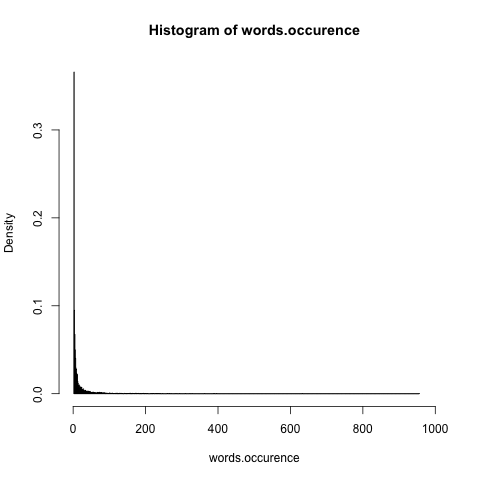
\includegraphics[width=0.5\textwidth]{img/hist.png}
\captionof{figure}{Histogram}
\end{center}
\end{org}





\begin{minted}[frame=lines,linenos=true]{r}
round(t(quantile(words.occurence,  probs = c(0, 25, 50, 75, 100)/100)))
\end{minted}

\begin{org}
\begin{center}
\captionof{table}{Quantiles}
\begin{tabular}{rrrrr}
0\% & 25\% & 50\% & 75\% & 100\%\\
\hline
2 & 3 & 5 & 14 & 17316\\
\end{tabular}
\end{center}
\end{org}




\textbf{1.2}

\begin{minted}[frame=lines,linenos=true]{r}
source("script2_HW6.R")
words <- colnames(dtm.mat)
words.occurence <- colSums(dtm.mat)
top.ten <- t(words[order(words.occurence, decreasing=T)[1:10]])
\end{minted}

\begin{org}
\begin{center}
\captionof{table}{Most used words with reparametrization}
\begin{tabular}{llllllllll}
she & her & music & econom & law & scienc & mathemat & new & histori & research\\
\end{tabular}
\end{center}
\end{org}




\textbf{1.3}

\begin{org}
\begin{center}
\captionof{table}{Dimensions after removing most common words}
\begin{tabular}{rr}
Number of individuals & Number of words\\
\hline
812 & 6653\\
\end{tabular}
\end{center}
\end{org}





\begin{minted}[frame=lines,linenos=true]{r}
words <- colnames(dtm.mat.raw)
words.occurence <- colSums(dtm.mat.raw)
top.ten <- t(words[order(words.occurence, decreasing=T)[1:10]])
\end{minted}

\begin{org}
\begin{center}
\captionof{table}{Most used words after removing the most common}
\begin{tabular}{llllllllll}
she & her & econom & polit & law & music & mathemat & theori & physic & play\\
\end{tabular}
\end{center}
\end{org}




\textbf{1.4}

\begin{minted}[frame=lines,linenos=true]{r}
ben.id <- which(dat$name == "Ben Bernanke")
#dat[ben.id,]
\end{minted}


\begin{quote}
ben shalom bernanke brnki brnangkee born december 13 1953 is an american economist at the brookings institution who served two terms as chairman of the federal reserve the central bank of the united states from 2006 to 2014 during his tenure as chairman bernanke oversaw the federal reserves response to the late2000s financial crisisbefore becoming federal reserve chairman bernanke was a tenured professor at princeton university and chaired the department of economics there from 1996 to september 2002 when he went on public service leavefrom 2002 until 2005 he was a member of the board of governors of the federal reserve system proposed the bernanke doctrine and first discussed the great moderation the theory that traditional business cycles have declined in volatility in recent decades through structural changes that have occurred in the international economy particularly increases in the economic stability of developing nations diminishing the influence of macroeconomic monetary and fiscal policybernanke then served as chairman of president george w bushs council of economic advisers before president bush nominated him to succeed alan greenspan as chairman of the united states federal reserve his first term began february 1 2006 bernanke was confirmed for a second term as chairman on january 28 2010 after being renominated by president barack obama his second term ended february 1 2014 when he was succeeded by janet yellen
\end{quote}



\begin{minted}[frame=lines,linenos=true]{r}
ben.id <- which(dat$name == "Ben Bernanke")
top.ten <- function(row) order(row, decreasing=T)[1:10]
list(1:10,
colnames(dtm.mat)[top.ten(dtm.mat[ben.id,])],
colnames(dtm.mat.raw)[top.ten(dtm.mat.raw[ben.id,])])
\end{minted}

\begin{org}
\begin{center}
\captionof{table}{Most common word}
\begin{tabular}{rll}
rank & dtm.mat & dtm.mat.raw\\
\hline
1 & bernank & chairman\\
2 & reserv & bernank\\
3 & chairman & feder\\
4 & feder & reserv\\
5 & term & term\\
6 & bush & econom\\
7 & succeed & bush\\
8 & econom & februari\\
9 & janet & second\\
10 & volatil & tenur\\
\end{tabular}
\end{center}
\end{org}


\textbf{1.5}


\begin{minted}[frame=lines,linenos=true]{r}
# Renormalize
dtm.mat.norm <- t(quick.norm(t(dtm.mat), mod=1))

# K-means algorithm
library(akmeans)
set.seed(10)
res <- norm.sim.ksc(dtm.mat.norm, k=8)
list(1:8, res$size)
\end{minted}

\begin{org}
\begin{center}
\captionof{table}{Clusters size}
\begin{tabular}{rr}
cluser & size\\
\hline
1 & 64\\
2 & 71\\
3 & 55\\
4 & 205\\
5 & 117\\
6 & 52\\
7 & 109\\
8 & 139\\
\end{tabular}
\end{center}
\end{org}



\begin{minted}[frame=lines,linenos=true]{r}
top.words.in.cluster <- function(i){
    individuals <- which(res$cluster == i)
    words <- colnames(dtm.mat.raw)
    count <- colSums(dtm.mat.raw[individuals, ])
    top.25 <- t(words[order(count, decreasing=T)[1:25]])

    c(i,top.25)
}

sapply(1:8, top.words.in.cluster)
\end{minted}

\begin{org}
\begin{center}
\captionof{table}{Top 25 words in each cluster}
\begin{tabular}{llllllll}
1 & 2 & 3 & 4 & 5 & 6 & 7 & 8\\
she & physic & she & she & music & polit & she & she\\
econom & theori & her & polit & she & her & her & her\\
her & mathemat & team & econom & her & she & econom & law\\
theori & she & coach & law & play & modern & literatur & then\\
develop & her & play & her & polit & jewish & mathemat & board\\
physic & field & band & program & perform & philosophi & review & play\\
comput & prize & season & board & team & war & journal & develop\\
mathemat & theoret & their & polici & orchestra & econom & editor & human\\
law & quantum & music & affair & festiv & visit & english & career\\
advanc & music & assist & educ & record & california & law & washington\\
california & develop & record & former & econom & european & theolog & name\\
engin & string & head & committe & mathemat & german & critic & team\\
geolog & known & high & social & theori & yale & languag & use\\
polit & comput & jersey & offic & compos & their & teach & foundat\\
press & philosophi & album & develop & symphoni & advanc & write & into\\
then & then & citi & journal & prize & press & taught & mani\\
area & use & theolog & appoint & london & histor & cultur & were\\
had & california & career & secur & visit & germani & theori & won\\
join & engin & design & washington & ensembl & historian & press & citi\\
use & mani & game & foundat & physic & physic & former & had\\
astronomi & under & had & join & law & recent & human & but\\
career & general & hockey & elect & press & under & music & journal\\
church & medal & began & assist & program & comput & prize & sever\\
best & high & more & dure & comput & later & scholar & jersey\\
dure & law & name & senat & women & law & articl & prize\\
\end{tabular}
\end{center}
\end{org}






\begin{minted}[frame=lines,linenos=true]{r}
p <- c(0, 1, 25, 50, 75, 100)
quantile.words.in.cluster <- function(i){
        individuals <- which(res$cluster == i)
        words <- colnames(dtm.mat.raw)
        count <- colSums(dtm.mat.raw[individuals, ])
        count <- count[count > 0]
        q <- quantile(count,  probs=p/100)
        c(i, round(q))
    }

    cbind(c("Cluster", paste(p, "%", sep="")), sapply(1:8, quantile.words.in.cluster))
\end{minted}

\begin{org}
\begin{center}
\captionof{table}{Quantiles in each cluster}
\begin{tabular}{lrrrrrrrr}
Cluster & 1 & 2 & 3 & 4 & 5 & 6 & 7 & 8\\
0\% & 1 & 1 & 1 & 1 & 1 & 1 & 1 & 1\\
1\% & 1 & 1 & 1 & 1 & 1 & 1 & 1 & 1\\
25\% & 1 & 1 & 1 & 1 & 1 & 1 & 1 & 1\\
50\% & 2 & 2 & 2 & 2 & 2 & 2 & 2 & 2\\
75\% & 4 & 4 & 4 & 6 & 4 & 3 & 4 & 5\\
100\% & 80 & 110 & 89 & 223 & 234 & 47 & 144 & 110\\
\end{tabular}
\end{center}
\end{org}




\section{Q2}
\label{sec:orgheadline4}

\begin{align*}
\log P(X, \psi)
&= \sum_i P(X_i; \psi)
\\&= \sum_i \sum_{j} P(X_i, Z_i = j; \psi)
\\&= \sum_i \sum_{j} \gamma_{ij}^{(t)} \frac{\log P(X_i, Z_i = j; \psi)}{\gamma_{ij}^{(t)}}
&(\gamma_{ij}^{(t)} = P(Z_i = j | X_i ; \psi^{(t)}))
\\&\ge \sum_{i, j}  \gamma_{ij}^{(t)} \frac{\log P(X_i, Z_i = j; \psi)}{\gamma_{ij}^{(t)}}
\\&= \sum_{i,j}  \gamma_{ij}^{(t)} \log P(X_i, Z_i = j; \psi) + cte
\\&= \sum_{i,j}  \gamma_{ij}^{(t)} \log \eta_j e^{- \frac{||X_i - \theta_j||_2^2}{2\sigma_j^2}} + cte
\\&= \sum_{j}  (\sum_i \gamma_{ij}^{(t)}) \log \eta_j - \sum_{ij} \gamma_{ij}^{(t)} \frac{||X_i - \theta_j||_2^2}{2\sigma_j^2} + cte
\end{align*}


With
\[\gamma_{ij}^{(t)} = \frac{\eta_j^{(t)} p_{\theta^{(t)}_j}(X_i)}{\sum_k \eta_k^{(t)} p_{\theta^{(t)}_k}(X_i)} = \frac{\eta_j^{(t)} e^{- \frac{||X_i - \theta_j||_2^2}{2\sigma_j^2}}}{\sum_k \eta_k^{(t)} e^{- \frac{||X_i - \theta_k||_2^2}{2\sigma_k^2}}}
\underset{\sigma_{ij} 0}{\longrightarrow} \left\{\begin{array}{cc}
1 & \text{if $\theta_j$ is the closest center to $X_i$}\\
0 & \text{o.w.}
\end{array}
\right. := I(\theta_j, X_i)
\]



\subsubsection{Finding \(\eta\)}
\label{sec:orgheadline2}
\(\max_\eta \rightarrow \sum_{j}  (\sum_i \gamma_{ij}^{(t)}) \log \eta_j\) under the constraint \(\sum_j \eta_j = 1\)
Lagragian: \(L(\eta, \lambda) = \sum_{j}  (\sum_i \gamma_{ij}^{(t)}) \log \eta_j + \lambda(1- \sum_j \eta_j)\)
-- \(\partial_{\eta_j} L = 0 \implies \sum_i \gamma_{ij}^{(t)} = \lambda \eta_j\)
-- \(\sum_j \eta_j = 1 \implies \lambda = \sum_{ij}\gamma_{ij}^{(t)} = n\) 
--
\begin{align*}
\eta_j^{(t+1)} = \frac{\sum_i \gamma_{ij}^{(t)}}n \rightarrow \frac{\#\{\text{number of $x_i$ close to $\theta_j$}\}}{n}
\end{align*}

\subsubsection{Finding \(\theta, \sigma\)}
\label{sec:orgheadline3}
\(L(\theta, \sigma) = - \sum_{ij} \gamma_{ij}^{(t)} \frac{||X_i - \theta_j||_2^2}{2\sigma_j^2}\)
-- \(\partial_{\theta_j} L = 0 \implies \sum_i \gamma_{ij}^{(t)} \frac{X_i - \theta_j}{\sigma_j^2} = 0\),
-- $$\theta_j = \frac{\sum_i \gamma_{ij}^{(t)} X_i}{\sum_i \gamma_{ij}^{(t)}} \rightarrow \frac{\sum_i I(\theta_j^{(t)}, X_i) X_i}{\sum_i I(\theta_j^{(t)}, X_i)} $$


\section{Q3}
\label{sec:orgheadline5}

\textbf{3.1}

Notation:

\(\alpha_i(t) = P(X_1, \ldots X_t, Z_t = i)\)
\(\beta_i(t) = P(X_{t+1}, \ldots X_n | Z_t = i)\)
\(\gamma_i(t) = P(Z_t = i | X)\)
\(p_j(x)\)  the density of \(\mathcal N(\mu_j, \Sigma_j)\)

Markov property:  
$$P(X, Z | \psi) = \eta_{Z_1} \prod_{t=1}^n A_{z_{t-1}q_t} p_{z_t}(X_t)$$
So:
\begin{align*}
Q(\psi, \psi^{old}) &= \sum_{Z \in [0, k-1]^n} \log P(X, Z | \psi) P(X, Z | \psi^{old})
\\&=
\underbrace{\sum_{Z \in [0, k-1]^n} \log \eta_{Z_1} P(X, Z | \psi^{old})}_{f_1(\eta)}
+ \underbrace{\sum_Z \left( \sum_{t=2}^n \log A_{Z_{t-1}Z_t}\right) P(X, Z | \psi^{old})}_{f_2(A)}
+ \underbrace{\sum_Z \left( \sum_{t=2}^n \log p_{Z_t}(X_t) \right) P(X, Z | \psi^{old})}_{f_3(\mu, \Sigma)}
\end{align*}

We can optimze each one of the \(f_r, r=1\ldots3\) independently.

\begin{itemize}
\item \(f_1(\eta) = \sum_{Z_1} \log \eta_{Z_1} \sum_{Z_2, \ldots Z_n} P(X, Z_1, \ldots Z_n | \psi^{old}) = \sum_{j} \log \eta_j P(X, Z_1=j | \psi^{old})\)
\end{itemize}
We maximize \(f_1\) under the constraint that \(\sum_j \eta_j = 1\). Noting \(\lambda\) the lagrage multiplier, the first order condition gives:
\(\frac1{\eta_j} P(X, Z_1 = j | \psi^{old}) = \lambda \; \forall j=0\ldots k-1\), eg \(\eta_j \propto P(X, Z_1 = j | \psi^{old}) \propto P(Z_1 = j | X, \psi^{old})\).
Since the \(\eta_j\) sum up to one:
$$\eta_j \leftarrow  \frac{P(Z_1 = j | X, \psi^{old})}{\sum_r P(X, Z_1 = r | X, \psi^{old})}$$

\begin{itemize}
\item We maximize
\begin{align*}
f_2(A)
&= \sum_{t=2}^n \sum_{Z_{t-1}, Z_t} \log A_{Z_{t-1}, Z_t} \left(\sum_{Z_1 \ldots Z_{t-2}, Z_{t+1}, \ldots Z_n} P(X, Z | \psi^{old})\right)
\\&= \sum_{t=2}^n \sum_{Z_{t-1}=s, Z_t=r} \log A_{s, r}  P(X, Z_{t-1}=s, Z_t=r | \psi^{old})
\end{align*}
\end{itemize}


Under the constraint that for all \(s\), \(\sum_r A_{sr} = 1\)


In a similar way, KKT condition give 

$$A_{sr} \leftarrow \frac{\sum_{t=2}^n P(Z_{t-1} = s, Z_t = r | X, \psi^{old})}{\sum_{j=0}^{k-1}\sum_{t=2}^n P(Z_{t-1} = s, Z_t = j | X, \psi^{old})}$$

\begin{itemize}
\item We maximize
\end{itemize}

\begin{align*}
f_3(\mu, \Sigma) &= \sum_{t=2}^n \sum_{Z_t=j} \log p_j(X_t)  \sum_{Z_i, i \neq t} P(X, Z | \psi^{old})
\\&= \sum_{t=2}^n \sum_{Z_t=j} \log p_j(X_t)  P(X, Z_t | \psi^{old})
\\&\propto - \sum_{Z_t=j} \sum_{t=2}^n \underbrace{P(X, Z_t=j | \psi^{old})}_{\gamma_{jt}} \left((X_t - \mu_j)'\Sigma_j^{-1}(X_t - \mu_j) +  \log(|\Sigma_j|)\right)
\\&\propto - \sum_{Z_t=j} tr\left(\Sigma_j^{-1} \underbrace{\sum_t \gamma_{jt} (X_t - \mu_j)'(X_t - \mu_j)}_{S_j}\right) +  \sum_j \left(\underbrace{\sum_t \gamma_{jt}}_{\gamma}\right) \log(|\Sigma_j|)
\end{align*}

First order conditions:
\begin{itemize}
\item \(0 = \frac{\partial}{\partial \mu_j} f_3 \implies \sum_t \gamma_{jt} (\mu_j - X_t)' \Sigma_j^{-1} = 0 \implies \mu_j = \frac{\sum_t \gamma_{jt}X_t}{\sum_t \gamma_{jt}}\)
\item \(0 = \frac{\partial}{\partial \Sigma_j^{-1}} f_3 \implies 2S_j - diag(S_j) + \gamma (2\Sigma_j - diag(\Sigma_j)) = 0 \implies 2(\gamma \Sigma_j-S_j) = diag(\gamma \Sigma_j-S_j) \implies \Sigma_j = \frac{S}{\gamma}\)
\end{itemize}

As a conclusion:

$$\Sigma_j \leftarrow \frac{\sum_t P(X, Z_t=j | \psi^{old}) (X_t - \mu_j)'(X_t - \mu_j)}{\sum_t P(X, Z_t=j | \psi^{old})}$$
$$\mu_j \leftarrow \frac{\sum_t P(X, Z_t=j | \psi^{old})X_t}{\sum_t P(X, Z_t=j | \psi^{old})}$$


\textbf{3.2}
Condition on \(Z_i\), \(X_{i+1}\ldots X_n\) is independent from \(X_1, \ldots X_{i}\), so:
\(\alpha(Z_i)\beta(Z_i) = P(X_1, \ldots X_i, Z_i | \psi) P(X_{i+1}, \ldots X_n| Z_i,  \psi) = P(X, Z_i | \psi)\)


\begin{align*}
P(Z_i | X_1, \ldots X_n, \psi)
&= \frac{P(X, Z_i | \psi)}{P(X | \psi)}
\\&= \frac{P(X, Z_i | \psi)}{\sum_{j} P(X, Z_i=j | \psi)}
\\&\propto \alpha(Z_i)\beta(Z_i)
\end{align*}



\begin{align*}
&P(X_i | Z_i, \psi) \sum_{Z_{i=1} = r} \alpha(Z_{i-1}) P(Z_i | Z_{i-1}=r, \psi)
\\&= \sum_{Z_{i-1} = r} P(X_i | Z_i, \psi) P(X_1, \ldots X_{i-1}, Z_{i-1}=r | \psi) P(Z_i | Z_{i-1}=r, \psi)
\\&= \sum_{Z_{i-1} = r}  P(X_1, \ldots X_{i-1}, Z_{i-1}=r | \psi) P(Z_i | Z_{i-1}=r, X_1, \ldots X_{i-1}, Z_{i-1}=r \psi) P(X_i | Z_i, X_1, \ldots X_{i-1}, Z_{i-1}=r, \psi) 
\\&\text{(Markov property)}
\\&= \sum_{Z_{i-1} = r}  P(X_1, \ldots X_{i-1}, X_i, Z_{i-1}=r, Z_i)
\\&= \alpha(Z_i)
\end{align*}




\begin{align*}
\beta(Z_i)
&= P(X_{i+1}\ldots X_n | Z_i)
\\&= \sum_{Z_{i+1}}P(X_{i+1}\ldots X_n | Z_i, Z_{i+1})P(Z_{i+1} | Z_i)
\\&= \sum_{Z_{i+1}}P(X_{i+2}\ldots X_n | Z_i, Z_{i+1})P(X_{i+1} | Z_{i+1})P(Z_{i+1} | Z_i)
\\&= \sum_{Z_{i+1}}\beta(Z_{i+1})P(X_{i+1} | Z_{i+1})P(Z_{i+1} | Z_i)
\end{align*}
\end{document}